\documentclass[11pt]{article}

% ---------------------------------------------------------------------------
% Supplementary Material: detailed model descriptions.
% Companion to manuscript.tex. Builds standalone (pdflatex supplementary.tex).
% ---------------------------------------------------------------------------
\usepackage[T1]{fontenc}
\usepackage[utf8]{inputenc}
\usepackage[a4paper,margin=2.4cm]{geometry}
\usepackage{graphicx}
\usepackage{amsmath}
\usepackage{booktabs}
\usepackage{caption}
\usepackage{longtable}
\usepackage[hidelinks]{hyperref}
\usepackage{xcolor}
\usepackage{titlesec}

\captionsetup{font=small,labelfont=bf}
\titleformat*{\section}{\large\bfseries}
\titleformat*{\subsection}{\normalsize\bfseries}
\setlength{\parskip}{0.4em}
\setlength{\parindent}{0pt}

% Number supplementary floats/sections with an S prefix
\renewcommand{\thesection}{S\arabic{section}}
\renewcommand{\thesubsection}{S\arabic{section}.\arabic{subsection}}
\renewcommand{\thefigure}{S\arabic{figure}}
\renewcommand{\thetable}{S\arabic{table}}
\renewcommand{\theequation}{S\arabic{equation}}

\title{\bfseries Supplementary Material\\[2pt]
\large A computational model of the interactions between formate and insulin
metabolism}
\author{Alexei Vazquez}
\date{Detailed model equations, parameters, calibration and numerical methods}

\begin{document}
\maketitle

\noindent This document gives the full technical specification of every model used
in the main text: state variables, rate laws, ODE balances, parameter values with
provenance, calibration procedures, and numerical methods. It is intended as a
complete and reproducible reference; the main text is kept to the biological
narrative and points here for detail. The model is implemented as an
object-oriented class hierarchy in \texttt{model.py} --- a \texttt{MetabolicCell}
base (shared numerics and rate-law primitives) subclassed by
\texttt{BetaCellModel}, \texttt{AdipocyteModel} and \texttt{EyeModel}, with
\texttt{WholeBody}, \texttt{FormateDiabetes}, \texttt{CoupledModel} and its
gut-microbiome extension \texttt{GutUrateCycle} containers,
each carrying an explicit parameter dataclass. All code, calibrated outputs
(\texttt{data/*.csv}) and figure scripts are in the accompanying repository.

\tableofcontents

% ===========================================================================
\section{Conventions and numerical methods}\label{sec:conv}

\textbf{Units.} Time is in hours; metabolite concentrations in mM; insulin and
lipid pools in arbitrary anabolic units (a.u.); plasma insulin in a.u. Blood
formate is reported in mM and, for clinical comparison, in mg/L using the formate
molecular weight $46.03$ (\mbox{mg/L $=$ mM $\times 46.03$}); blood urate in mg/dL
using $16.8$.

\textbf{Provenance tags.} Every parameter carries one of four tags.
\textbf{[PUB]} inherited from the previously published Formate--NUDT5 purine/energy
core (Vazquez, submitted); \textbf{[FIT]} fitted here by least squares to the
calibration targets of \S\ref{sec:betacal}; \textbf{[LIT]} taken from a specific
literature measurement; \textbf{[ASM]} assumed / order-of-magnitude estimate not
individually measured. Tags are given in the parameter tables.

\textbf{Integration.} All ODEs are integrated with an implicit
backward-differentiation (BDF) solver
(\texttt{scipy.integrate.\allowbreak solve\_ivp}) with dense output. Tolerances
are stated per model.

\textbf{Steady states.} Unless noted, a steady state is obtained by
pre-integrating to a physiologically reasonable basin and then polishing the
residual in log-space with \texttt{least\_squares} (variables $z=\log y$, residual
$\dot y(e^{z})/(e^{z}+10^{-6})$, so states stay positive), to residuals
$<10^{-13}$~mM/h. The one exception is the regulated eye feed-forward
(\S\ref{sec:eyeff}), where a steady state is obtained by integration to the stable
attractor rather than root-polishing, for reasons made precise in
\S\ref{sec:bif}.

% ===========================================================================
\section{The pancreatic $\beta$-cell model}\label{sec:beta}

The core is a fifteen-state kinetic model of the coupled energy, one-carbon,
purine, mTORC1 and insulin-synthesis network of a glucose-responsive
$\beta$-cell. The purine/energy backbone and the PPAT--NUDT5 ``glue'' calibration
are inherited from the Formate--NUDT5 model; the insulin-synthesis, secretion and
glucose-sensing layers are added and fitted here.

\subsection{State variables}
\begin{table}[h]\centering\small
\caption{The fifteen $\beta$-cell state variables (array order), with initial
condition $Y_0$.}
\begin{tabular}{@{}rlll r@{}}
\toprule
$i$ & symbol & meaning & units & $Y_{0,i}$\\
\midrule
0 & \texttt{atp} & ATP & mM & 3.0\\
1 & \texttt{adp} & ADP & mM & 0.3\\
2 & \texttt{amp} & AMP & mM & 0.03\\
3 & \texttt{form} & intracellular formate & mM & 0.3\\
4 & \texttt{cho} & 10-formyl-THF (10-CHO-THF) & mM & 0.01\\
5 & \texttt{prpp} & PRPP & mM & 0.1\\
6 & \texttt{gar} & GAR (glycinamide ribonucleotide) & mM & 0.02\\
7 & \texttt{aic} & AICAR & mM & 0.02\\
8 & \texttt{imp} & IMP (purine hub) & mM & 0.05\\
9 & \texttt{samp} & adenylosuccinate (S-AMP) & mM & 0.02\\
10 & \texttt{gnp} & guanine nucleotides & mM & 1.0\\
11 & \texttt{hx} & hypoxanthine/xanthine & mM & 0.02\\
12 & \texttt{urate} & urate & mM & 0.05\\
13 & \texttt{proins} & pro-insulin & a.u. & 1.0\\
14 & \texttt{ins} & mature insulin (granule pool) & a.u. & 5.0\\
\bottomrule
\end{tabular}
\end{table}

All states are floored at $10^{-12}$ before rate evaluation. A common dilution
constant $\mu = 1/240~\mathrm{h^{-1}}$ (\,$\approx$ ten-day pool renewal\,) applies
to most pools; \texttt{form}, \texttt{cho}, \texttt{hx} and \texttt{urate} carry no
dilution term.

\subsection{Energy metabolism}
Glucose $G$ sets a glucokinase gate and a fuel level; ATP is produced by
glycolysis and oxidative phosphorylation (each Michaelis--Menten in ADP), consumed
by an ATPase and by anabolism, and the adenine nucleotides equilibrate through
adenylate kinase:
\begin{align}
gk &= \frac{G^{h_{gk}}}{K_{gk}^{h_{gk}}+G^{h_{gk}}}, &
\mathrm{fuel} &= \mathrm{BASALFUEL}+(1-\mathrm{BASALFUEL})\,gk,\\
\mathrm{cox} &= \Big[1+(\mathrm{form}/K_i^{\mathrm{cox}})^2\Big]^{-1}\ (\text{else }1), &
v_{glyc} &= e_g\,\mathrm{fuel}\,\frac{adp}{E_g+adp},\\
v_{ox} &= e_o\,\mathrm{fuel}\,\frac{adp}{E_o+adp}\,\mathrm{cox}, &
v_{atpase} &= a\,\frac{atp}{A+atp},\\
r_{ak} &= k_{ak}\Big(adp^2-\frac{amp\cdot atp}{K_{ak}}\Big), &
v_{atp}^{\mathrm{prod}} &= v_{glyc}+v_{ox}.
\end{align}
The complex-IV factor $\mathrm{cox}$ is a formate inhibition of oxidative
phosphorylation used only in the (optional, weakly evidenced) methanol
complex-IV scenario; it is \emph{disabled by default} ($K_i^{\mathrm{cox}}=$ None
$\Rightarrow \mathrm{cox}=1$) and is switched off entirely in the main-text eye
analyses.

\subsection{One-carbon entry and de novo purine synthesis}
Formate is charged onto tetrahydrofolate and drives the two formyl-transfer steps
of purine ring assembly; the committed step (PPAT) is gated by the AMP/PRPP
``glue'' term $\theta$:
\begin{align}
\mathrm{thf}&=F_{tot}-cho, &
v_{fthfs}&=h\,\tfrac{form}{H+form}\,\tfrac{\mathrm{thf}}{F_{tot}}, &
\mathrm{onec}&=\tfrac{cho}{K_c+cho},\\
\theta&=f_N\,\tfrac{1+(amp/K_a)^{n}}{1+(amp/K_a)^{n}+prpp/K_{dP}}, &
v_{ppat}&=P_{max}\,\tfrac{prpp}{K_{prpp}+prpp}\,(1-\theta),\\
v_{gart}&=g_{max}\,\tfrac{gar}{K_g+gar}\,\mathrm{onec}, &
v_{atic}&=t_{max}\,\tfrac{aic}{K_t+aic}\,\mathrm{onec}.
\end{align}
$f_N\in[0,1]$ scales the NUDT5 glue strength ($f_N=0$ disables the AMP/PRPP
feedback). The glue parameters $K_a,n$ are fitted (\S\ref{sec:betacal}) to the
Witus \textit{et al.}\ PRPP IC$_{50}$ vs.\ AMP data.

\subsection{Purine interconversion, degradation and urate}
With adenylate ratio $adr=atp/adp$:
\begin{align}
v_{imp\to amp}&=k_{amp}^{\mathrm{syn}}\,imp\,adr, &
v_{samp\to amp}&=V_{max}^{samp}\,\frac{samp}{K_{samp}+samp}, &
v_{imp\to gmp}&=k_{gmp}^{\mathrm{syn}}\,imp\,adr,\\
v_{imp}^{\mathrm{deg}}&=k_{imp}^{\mathrm{deg}}\,imp, &
v_{amp}^{\mathrm{deg}}&=k_{amp}^{\mathrm{deg}}\,amp, &
v_{ade}^{\mathrm{turn}}&=k_{ade}^{\mathrm{turn}}\,atp,\\
v_{gnp}^{\mathrm{deg}}&=k_{gnp}^{\mathrm{deg}}\,gnp, &
v_{xo}&=k_{xo}\,\frac{hx}{K_{hx}+hx}, &
v_{urate}^{\mathrm{sec}}&=k_{urate}\,urate,
\end{align}
and a guanine-nucleotide usage $v_{gnp}^{\mathrm{use}}=k_{gnp}^{\mathrm{use}}\,gnp$.

\subsection{mTORC1 and insulin synthesis}
mTORC1 senses a guanine-weighted purine pool and the adenylate energy charge;
insulin transcription is glucose-driven; peptide synthesis multiplies the two;
maturation and an ATP/ADP-triggered secretion complete the granule cycle:
\begin{align}
P_{\mathrm{pool}}&=W_{\mathrm{ATP}}\,atp+gnp, &
ec&=\frac{atp+0.5\,adp}{atp+adp+amp},\\
\mathrm{mtor}&=\mathrm{mtor\_mult}\cdot
\frac{P_{\mathrm{pool}}^{h_{mp}}}{K_{mp}^{h_{mp}}+P_{\mathrm{pool}}^{h_{mp}}}\cdot
\frac{ec^{h_{ec}}}{K_{ec}^{h_{ec}}+ec^{h_{ec}}}, &
g_{tx}&=B_{TX}+(1-B_{TX})\frac{G^{h_G}}{K_{G}^{h_G}+G^{h_G}},\\
v_{\mathrm{ins}}^{\mathrm{syn}}&=k_{ins}\big(B_{M}+(1-B_{M})\,\mathrm{mtor}\big)\,g_{tx}\,\frac{aa}{K_{aa}+aa}, &
v_{mat}&=k_{mat}\,proins,\\
\mathrm{trig}&=B_{TR}+(1-B_{TR})\frac{(atp/adp)^{h_{tr}}}{K_{tr}^{h_{tr}}+(atp/adp)^{h_{tr}}}, &
v_{sec}&=k_{sec}\,ins\,\mathrm{trig}.
\end{align}
The ATP cost of anabolism is
$v_{atp}^{\mathrm{cost}}=\mathrm{cost}_{ins}\,v_{\mathrm{ins}}^{\mathrm{syn}}+\mathrm{cost}_{pur}\,v_{ppat}$.
The multiplier $\mathrm{mtor\_mult}$ (default 1; $0=$ Raptor knockout) and the
mTOR-independent floor $B_M$ set the mTORC1 dependence of insulin content
(fitted to Ni \textit{et al.}, \S\ref{sec:betacal}).

\subsection{ODE balances}
With the fluxes above (and the override arguments $f_{\mathrm{mito}}$, the
mitochondrial formate production; $f_N$; $\mathrm{mtor\_mult}$; $K_i^{\mathrm{cox}}$
described in-line), the state derivatives are:
\begin{align}
\dot{atp}&=v_{atp}^{\mathrm{prod}}-v_{atpase}-v_{atp}^{\mathrm{cost}}+r_{ak}-v_{ade}^{\mathrm{turn}}-\mu\,atp,\\
\dot{adp}&=-v_{atp}^{\mathrm{prod}}+v_{atpase}+v_{atp}^{\mathrm{cost}}-2r_{ak}-\mu\,adp,\\
\dot{amp}&=r_{ak}+v_{samp\to amp}-v_{amp}^{\mathrm{deg}}-\mu\,amp,\\
\dot{form}&=f_{\mathrm{mito}}+k_F\,(\mathrm{form}_x-form)-v_{fthfs},\\
\dot{cho}&=v_{fthfs}-v_{gart}-v_{atic},\\
\dot{prpp}&=S_{prpp}-v_{ppat}-k_{o}^{prpp}\,prpp-\mu\,prpp,\\
\dot{gar}&=v_{ppat}-v_{gart}-(\mu+k_{\mathrm{deg}}^{\mathrm{int}})\,gar,\\
\dot{aic}&=v_{gart}-v_{atic}-(\mu+k_{\mathrm{deg}}^{\mathrm{int}})\,aic,\\
\dot{imp}&=v_{atic}-v_{imp\to amp}-v_{imp\to gmp}-v_{imp}^{\mathrm{deg}}-\mu\,imp,\\
\dot{samp}&=v_{imp\to amp}-v_{samp\to amp}-\mu\,samp,\\
\dot{gnp}&=v_{imp\to gmp}-v_{gnp}^{\mathrm{deg}}-v_{gnp}^{\mathrm{use}}-\mu\,gnp,\\
\dot{hx}&=v_{imp}^{\mathrm{deg}}+v_{amp}^{\mathrm{deg}}+v_{ade}^{\mathrm{turn}}+v_{gnp}^{\mathrm{deg}}-v_{xo},\\
\dot{urate}&=v_{xo}-v_{urate}^{\mathrm{sec}},\\
\dot{proins}&=v_{\mathrm{ins}}^{\mathrm{syn}}-v_{mat}-\mu\,proins,\\
\dot{ins}&=v_{mat}-v_{sec}-\mu\,ins.
\end{align}
Here $\mathrm{form}_x$ is the blood formate seen by the cell and $f_{\mathrm{mito}}$
(default FMITO) the endogenous mitochondrial formate; lowering $f_{\mathrm{mito}}$
represents MTHFD1L loss / mitochondrial formate deficiency.

\subsection{Parameters}
\begin{longtable}{@{}llll@{}}
\caption{$\beta$-cell parameters. Derived values expanded numerically
($m{=}84$, $e{=}2m{=}168$, $v_{pur}{=}0.30$).}\label{tab:betaparams}\\
\toprule
symbol & value & meaning & tag\\
\midrule
\endfirsthead
\multicolumn{4}{l}{\small\itshape Table~\thetable\ (continued)}\\
\toprule symbol & value & meaning & tag\\ \midrule
\endhead
\multicolumn{4}{c}{\textit{Energy / adenine nucleotides}}\\
$K_{gk}$ & 8.0 mM & glucokinase half-saturation & [LIT]\\
$h_{gk}$ & 1.7 & glucokinase Hill coefficient & [LIT]\\
$m$ & 84 mM/h & maintenance ATP turnover & [PUB]\\
$e$ & 168 mM/h & total ATP-cycling scale ($2m$) & [PUB]\\
$e_g$ & 100.8 mM/h & max glycolytic ATP rate ($0.6e$) & [PUB]\\
$e_o$ & 67.2 mM/h & max OxPhos ATP rate ($0.4e$) & [LIT]\\
BASALFUEL & 0.40 & glucose-independent fuel floor & [FIT]\\
$E_g,E_o$ & 0.25,\,0.12 mM & glycolysis/OxPhos ADP half-sat & [PUB]\\
$a$ & 168 mM/h & max ATPase rate & [FIT]\\
$A$ & 2.0 mM & ATPase half-saturation for ATP & [PUB]\\
$K_{ak}$ & 0.8 & adenylate-kinase equilibrium & [PUB]\\
$k_{ak}$ & $5\times10^{3}$/h & adenylate-kinase relaxation rate & [ASM]\\
\midrule
\multicolumn{4}{c}{\textit{One-carbon / de novo purine}}\\
$F_{tot}$ & 0.02 mM & cytosolic folate pool & [ASM]\\
$H$ & 0.01 mM & FTHFS half-sat for formate & [PUB]\\
$K_c$ & 0.002 mM & GART/ATIC half-sat for CHO-THF & [ASM]\\
$K_g,K_t$ & 0.01 mM & GART/ATIC half-sat for GAR/AICAR & [ASM]\\
$v_{pur}$ & 0.30 mM/h & resting purine-turnover scale & [ASM]\\
$h$ & 1.2 mM/h & FTHFS capacity ($4v_{pur}$) & [ASM]\\
$k_F$ & 0.625/h & formate exchange coefficient & [PUB]\\
FMITO & 0.5 mM/h & mitochondrial formate capacity & [ASM]\\
$P_{max},S_{prpp}$ & 0.6 mM/h & PPAT capacity / PRPP supply ($2v_{pur}$) & [ASM]\\
$K_{prpp}$ & 0.3 mM & PPAT half-saturation for PRPP & [ASM]\\
$k_o^{prpp}$ & 2.0/h & lumped PRPP drain & [ASM]\\
$g_{max},t_{max}$ & 1.5 mM/h & GART/ATIC capacity ($5v_{pur}$) & [ASM]\\
$k_{\mathrm{deg}}^{\mathrm{int}}$ & 0.1/h & GAR/AICAR intermediate drain & [ASM]\\
$K_{dP}$ & 0.104 mM & glue PRPP IC$_{50}$ at zero AMP & [FIT]\\
$K_a,n$ & fitted & glue AMP half-sat / Hill & [FIT]\\
\midrule
\multicolumn{4}{c}{\textit{Purine branch, degradation, urate}}\\
$k_{amp}^{\mathrm{syn}},k_{gmp}^{\mathrm{syn}}$ & 2.0 & ADSS / IMPDH mass-action (per $adr$) & [ASM]\\
$V_{max}^{samp}$ & 0.6 mM/h & ADSL capacity (S-AMP$\to$AMP) & [FIT]\\
$K_{samp}$ & 0.02 mM & ADSL half-saturation & [ASM]\\
$k_{imp}^{\mathrm{deg}}$ & 1.0/h & IMP degradation & [ASM]\\
$k_{amp}^{\mathrm{deg}}$ & 0.5/h & AMP degradation & [ASM]\\
$k_{ade}^{\mathrm{turn}}$ & 0.03/h & adenylate catabolism & [ASM]\\
$k_{gnp}^{\mathrm{deg}}$ & 0.5/h & GXP degradation & [ASM]\\
$k_{gnp}^{\mathrm{use}}$ & 0.3/h & guanine-nucleotide usage & [ASM]\\
$K_{hx}$ & 0.02 mM & xanthine-oxidase half-saturation & [ASM]\\
$k_{xo}$ & 0.6 mM/h & XOR capacity ($2v_{pur}$) & [LIT]\\
$k_{urate}$ & 3.0/h & urate secretion/export & [ASM]\\
\midrule
\multicolumn{4}{c}{\textit{mTOR / insulin synthesis / secretion}}\\
$W_{\mathrm{ATP}}$ & 0.03 & ATP weight in mTOR purine signal & [ASM]\\
$K_{mp},h_{mp}$ & 0.12 mM,\,2.0 & mTOR purine-sensing half-sat / Hill & [ASM]\\
$K_{ec},h_{ec}$ & 0.85,\,4.0 & energy-charge gate half-sat / Hill & [ASM]\\
$aa,K_{aa}$ & 2.0,\,0.5 mM & amino-acid pool / translation half-sat & [ASM]\\
$K_{G},h_{G}$ & 7.0 mM,\,2.0 & glucose insulin-gene half-max / Hill & [FIT]/[LIT]\\
$B_{TX}$ & 0.10 & basal insulin-gene drive & [FIT]\\
$B_{M}$ & 0.29 & mTOR-independent insulin fraction & [FIT]\\
$k_{ins}$ & 20 a.u./h & max pro-insulin synthesis rate & [ASM]\\
$k_{mat}$ & 3.0/h & pro-insulin maturation & [LIT]\\
$\mathrm{cost}_{ins}$ & 0.02 & ATP per a.u.\ insulin & [ASM]\\
$\mathrm{cost}_{pur}$ & 4.0 & ATP per mM purine & [LIT]\\
$K_{tr},h_{tr}$ & 12.0,\,4.0 & secretion-trigger half-sat / Hill (ATP/ADP) & [ASM]\\
$B_{TR}$ & 0.05 & basal secretion & [ASM]\\
$k_{sec}$ & 6.0/h & max fractional granule secretion & [LIT]\\
$\mu$ & 1/240\,/h & pool-renewal dilution & [ASM]\\
\bottomrule
\end{longtable}

\subsection{Calibration}\label{sec:betacal}
\texttt{recalibrate\_all()} fits the added layers in dependency order (energy
$\to$ IMP branch $\to$ mTOR/\allowbreak content $\to$ GSIS), each by \texttt{least\_squares} on
log-ratio residuals against independent targets, all evaluated at blood formate
$0.3$~mM:
\begin{enumerate}\itemsep1pt
\item \textbf{Energy} — fit BASALFUEL and ATPase capacity $a$ so ATP/ADP rises
$2.4\to11.6$ as glucose goes $1\to10$~mM (Detimary 1998).
\item \textbf{IMP branch} — fit the ADSL capacity $V_{max}^{samp}$ so S-AMP rises
$\times3.4$ over glucose $2.8\to16.7$~mM (Gooding 2015); the accompanying IMP fall
($\sim{-}75\%$ vs.\ target $-77\%$) is structural, not fitted.
\item \textbf{mTOR / content} — fit the floor $B_M$ so a full mTORC1 knockout
($\mathrm{mtor\_mult}{=}0$) gives $50\%$ of wild-type insulin content (Ni 2017).
\item \textbf{GSIS} — fit the glucose half-max $K_G$ and basal drive $B_{TX}$ to a
secretion EC$_{50}$ of $8.0$~mM and a stimulation index of $5.5$; $K_G$ bounded to
$[4,12]$~mM (glucokinase-linked plausibility).
\end{enumerate}
Absolute per-cell units are set by one scale anchoring the granule pool at
stimulatory glucose to the measured $\beta$-cell insulin content ($20$~pg/cell);
all calibrated ratios (EC$_{50}$, stimulation index, formate sensitivity) are
invariant under it. Steady states use the pre-integration ($t_{\mathrm{pre}}=150$~h)
plus log-space polish of \S\ref{sec:conv}; trajectory integration uses BDF with
$\mathrm{rtol}=10^{-8}$, $\mathrm{atol}=10^{-10}$.

% ===========================================================================
\section{Whole-body loop (Bergman minimal model)}\label{sec:wb}

The $\beta$-cell is embedded as the insulin source of a Bergman minimal model.
The coupled state is $[\,y_{bc},\,G_b,\,I_p,\,X\,]$: blood glucose $G_b$, plasma
insulin $I_p$, and remote (interstitial) insulin action $X$. With effective
glucose effectiveness $S_g^{\mathrm{eff}}=S_g(1+\mathrm{peri})$,
\begin{align}
\dot G_b&=R_a(t)-\big(S_g^{\mathrm{eff}}+X\big)G_b+S_g^{\mathrm{eff}}G_{b0},\\
\dot I_p&=\beta\,v_{sec}(y_{bc},G_b,\mathrm{form}_x,f_N)-k_I\,I_p,\\
\dot X&=-p_2 X+p_2 S_i\,(I_p-I_{b,\mathrm{ref}}),\\
\dot y_{bc}&=\text{$\beta$-cell derivatives at glucose }G_b.
\end{align}
Insulin secretion is evaluated at the current blood glucose, closing the
glucose$\to$insulin$\to$glucose loop. \emph{Central} formate acts through the
$\beta$-cell arguments $\mathrm{form}_x$ and $f_{\mathrm{mito}}$ (raising $v_{sec}$);
the \emph{peripheral} (Carpene) effect enters only as the insulin-independent
fractional boost $\mathrm{peri}$ to glucose effectiveness. Parameters (per hour):
$G_{b0}=5.0$~mM [LIT], $S_g=1.5$ [LIT], $p_2=1.2$ [LIT], $S_i=1.0$ [ASM],
$k_I=30$ [LIT], $\beta=10$ [ASM]; the remote-action gain uses $p_2 S_i$ in place
of the classical $p_3$. Basal insulin is $I_b=\beta v_{sec}/k_I$.

\textbf{Central-vs-peripheral discriminator.} A four-arm intravenous glucose
tolerance test (bolus $8$~mM, $R_a=0$, integrated $4$~h, BDF $10^{-7}/10^{-9}$)
compares a formate-deficient baseline ($f_{\mathrm{mito}}=0.2\,$FMITO), a central
arm ($f_{\mathrm{mito}}=$ FMITO), a peripheral arm ($\mathrm{peri}=0.30$, tuned to
match the central glucose improvement), and both. Outputs are glucose AUC above
$G_{b0}$ and total insulin AUC; both arms lower glucose AUC, but only the central
arm raises insulin AUC ($>5\%$ classifies ``central-like'').

% ===========================================================================
\section{Blood-formate dynamics (diabetes paradox)}\label{sec:fd}

To ask how circulating formate itself moves, a dynamic blood-formate pool $F_b$ is
added to the fasting whole-body loop ($R_a=0$), and the $\beta$-cell now draws its
formate from $F_b$ (closing the formate$\to$insulin$\to$formate loop). A secretion
defect $s\in[0,1]$ scales insulin appearance:
\begin{align}
\dot G_b&=-\big(S_g+X\big)G_b+S_g G_{b0}, &
\dot I_p&=\beta\,s\,v_{sec}-k_I I_p,\\
\dot X&=-p_2X+p_2S_i(I_p-I_{b,\mathrm{ref}}), &
\mathrm{ins\_frac}&=\tfrac{I_p}{K_I+I_p},\\
U_{\mathrm{form}}&=\big(U_0+U_{\mathrm{ins}}\,\mathrm{ins\_frac}\big)\tfrac{F_b}{K_F+F_b}, &
\dot F_b&=D_{\mathrm{diet}}+P_{\mathrm{endog}}-U_{\mathrm{form}}-k_{\mathrm{ren}}F_b.
\end{align}
Blood formate is produced by diet ($D_{\mathrm{diet}}$) and endogenous synthesis
($P_{\mathrm{endog}}$) and drained by an insulin-scaled, formate-saturating
anabolic sink $U_{\mathrm{form}}$ (purine synthesis, the main sink) and renal
clearance. Parameters (mM, per hour): $P_{\mathrm{endog}}=0.02$, $k_{\mathrm{ren}}=0.5$,
$U_0=0.01$, $U_{\mathrm{ins}}=0.12$, $K_F=0.05$ [all ASM]; the insulin half-sat
$K_I$ is pinned to the healthy basal plasma insulin (sink half-engaged at health).
Dietary intakes (mM/h): low $0.010$, normal $0.030$, high $0.080$. Sweeping the
secretion defect $s:1.0\to0.15$ shows that a secretion defect \emph{raises} blood
formate (reduced insulin-driven consumption): the overflow route by which incident
diabetes can carry higher circulating formate.

% ===========================================================================
\section{Adipocyte model and three-compartment obesity/diabetes coupling}\label{sec:adip}

\subsection{Adipocyte (ten ODEs)}
The adipocyte reuses the energy and one-carbon/\allowbreak purine machinery of the
$\beta$-cell but replaces insulin peptide synthesis with insulin-driven lipid
storage, and is XOR-rich (a urate source). The state and its initial condition are
\[
[\,atp,adp,amp,form,cho,imp,gnp,hx,urate,lipid\,],
\]
\[
Y_0=[\,2.0,0.2,0.03,0.3,0.01,0.05,0.1,0.02,0.05,5.0\,].
\]
Insulin-dependent GLUT4 uptake, the formate sink, the XOR/\allowbreak urate arm and
lipogenesis are:
\begin{align}
\mathrm{ins\_glut}&=B_{GLUT}+(1-B_{GLUT})\tfrac{I}{K_{Iglut}+I}, &
\mathrm{uptake}&=\mathrm{ins\_glut}\,\tfrac{G}{K_{glut}+G},\\
v_{fthfs}&=h_A\tfrac{form}{H+form}\tfrac{\mathrm{thf}}{F_{tot}}, &
v_{xo}&=\mathrm{xor\_mult}\;k_{xo,a}\tfrac{hx}{K_{hx}+hx},\\
v_{lipo}&=k_{lipo}\tfrac{I}{K_{Ilipo}+I}\,\mathrm{uptake},\\
v_{denovo}&=V_{purA}\tfrac{prpp_a}{K_{prpp,a}+prpp_a}\,\mathrm{onec}\,(0.3+0.7\,\mathrm{uptake}),
\end{align}
with hypoxanthine also exported/salvaged ($v_{hx}^{\mathrm{exp}}=k_{hxexp}\,hx$,
competing with XOR) and urate secreted to blood ($k_{urate,a}\,urate$). Selected
parameters: $e_{adip}=1.2m=100.8$, $K_{glut}=5.0$~mM, $K_{Iglut}=0.5$,
$B_{GLUT}=0.10$; $v_{pur,a}=0.30$, $h_A=1.2$, $V_{purA}=0.6$, $prpp_a=0.3$~mM;
$k_{xo,a}=0.9$~mM/h (adipose is XOR-rich, Tsushima 2013), $k_{hxexp}=6.0$/h,
$k_{urate,a}=3.0$/h; $k_{lipo}=4.0$, $K_{Ilipo}=0.5$, $k_{lps}=0.2$/h,
$\mathrm{cost}_{lip}=0.03$; $\mu_a=1/240$/h [all ASM except $k_F=0.625$ PUB]. Two
one-carbon units are consumed per purine ($\dot{cho}=v_{fthfs}-2v_{denovo}$).

\subsection{Three-compartment coupling}
The full state is $[\,\text{$\beta$-cell (15)},\,\text{adipocyte (10)},\,G_b,I_p,X,F_b,U_b\,]$
with blood glucose, plasma insulin, remote action, blood formate and blood urate.
The $\beta$-cell and adipocyte are integrated as single cells whose net blood
exchange is scaled by adipose mass $M_{adip}$ and a tissue$\to$blood coupling
$c_{adip}=0.16$. Blood formate and urate obey
\begin{align}
S_g^{\mathrm{eff}}&=S_g\cdot\mathrm{sg\_mult}, &
\dot G_b&=-(S_g^{\mathrm{eff}}+X)G_b+S_g^{\mathrm{eff}}G_{b0},\\
\dot I_p&=\beta\,s\,v_{sec}-k_I I_p, &
U_{\mathrm{syst}}&=\Big(U_0+U_{\mathrm{ins}}\tfrac{I_p}{K_I+I_p}\Big)\tfrac{F_b}{K_F+F_b},\\
\dot F_b&=D_{\mathrm{diet}}+P_{\mathrm{endog}}-U_{\mathrm{syst}}-c_{adip}M_{adip}\,J_F-k_{\mathrm{ren}}F_b,\\
\dot U_b&=c_{adip}M_{adip}\,J_U+U_0^{\mathrm{ur}}-k_{\mathrm{ren}}^{u}U_b.
\end{align}
where $J_F=k_F(F_b-\mathrm{form}_{ad})$ is the per-cell adipose formate uptake and
$J_U$ the per-cell adipose urate secretion; $U_0^{\mathrm{ur}}=0.06$~mM/h
(non-adipose urate), $k_{\mathrm{ren}}^{u}=0.3$/h. Integrated to $t=600$~h
(BDF $10^{-6}/10^{-9}$); the healthy lean fixed point self-consistently sets $K_I$
to basal insulin.

\subsection{Obesity, diabetes, supplementation and metformin}
\textbf{Obesity} acts on three handles at once: adipose mass
$M_{adip}=3$, XOR induction $\mathrm{xor\_mult}=2$, and insulin resistance
$S_i\to0.5\,S_i$. \textbf{Diabetes} acts only through the secretion defect $s=0.40$.
Obesity thus lowers blood formate (adipose sink $+$ XOR) and raises urate, while a
secretion defect raises blood formate (overflow) --- the two axes move formate in
opposite directions (Table~\ref{tab:obes}).
\textbf{Supplementation} sweeps dietary intake $D:0.01\to0.16$~mM/h with the
$\beta$-cell either formate-replete ($f_{\mathrm{mito}}=$ None, default) or
formate-deficient ($f_{\mathrm{mito}}=0.2\,$FMITO$=0.1$); only the deficient
$\beta$-cell is rescuable.
\textbf{Metformin} at dose $d\in[0,1]$ applies a dual action: a peripheral/AMPK
rise in glucose effectiveness $\mathrm{sg\_mult}=1+d$, and an SHMT2-type reduction
of both systemic and $\beta$-cell mitochondrial formate,
$P_{\mathrm{endog}}\to0.02(1-0.6d)$ and $f_{\mathrm{mito}}\to0.5(1-0.6d)$ --- so it
lowers glucose while also lowering formate and insulin.

\begin{table}[h]\centering\small
\caption{Committed 2$\times$2 clinical fixed points (\texttt{data/obesity\_diabetes.csv}),
normal diet.}\label{tab:obes}
\small\setlength{\tabcolsep}{4pt}%
\begin{tabular}{@{}lrrrrr@{}}
\toprule
scenario & glucose (mM) & insulin (a.u.) & formate (mg/L) & urate (mg/dL) & formate vs healthy\\
\midrule
lean, non-diabetic & 4.79 & 0.82 & 1.46 & 3.44 & 0\%\\
obese, non-diabetic & 4.87 & 0.84 & 1.25 & 3.57 & $-14\%$\\
lean, diabetic & 6.26 & 0.46 & 1.76 & 3.45 & $+21\%$\\
obese, diabetic & 5.67 & 0.40 & 1.53 & 3.61 & $+5\%$\\
\bottomrule
\end{tabular}
\end{table}

\subsection{Gut-microbiome urate cycle}\label{sec:gut}
The class \texttt{GutUrateCycle} extends the three-compartment model with a gut
compartment that degrades blood urate and returns formate to the circulation,
closing the delayed positive feedback of the urate-cycle hypothesis (Vazquez,
2020; gut purine metabolism after Kasahara \textit{et al}, 2023). Blood urate is
taken up by the gut route at rate $k_{gut}$ (diverting it from renal clearance)
and one of the two purine-derived formate carbons is returned as formate,
$Y_{\mathrm{form}}$ per urate. The gut processing/transit delay is a linear chain
of $n_{gut}$ compartments $g_1\dots g_{n_{gut}}$ with rate $k_g=n_{gut}/\tau_{gut}$
(the linear-chain trick for a gamma-distributed lag of mean $\tau_{gut}$):
\begin{align}
\dot U_b &\mathrel{+}= -\,k_{gut}\,U_b, &
\dot g_1 &= k_{gut}\,U_b - k_g\,g_1, &
\dot g_i &= k_g\,g_{i-1} - k_g\,g_i, &
\dot F_b &\mathrel{+}= Y_{\mathrm{form}}\,k_g\,g_{n_{gut}}.
\end{align}
At steady state the chain gives $k_g g_{n_{gut}}=k_{gut}U_b$, so the return flux is
$Y_{\mathrm{form}}k_{gut}U_b$ and the delay affects only the dynamics. Because only
one of the two formate carbons consumed per purine is recycled, the loop gain is
below one: blood formate rises and converges (bounded feedback) rather than
running away. Parameters (all [ASM]): $k_{gut}=0.2$/h, $Y_{\mathrm{form}}=1$,
$\tau_{gut}=12$~h, $n_{gut}=3$; the co-produced acetate ($\to$ lipogenesis) is
noted but not tracked. Generated by \texttt{make\_gutcycle.py}.

% ===========================================================================
\section{The eye compartment}\label{sec:eye}

The eye is a retinal insulin-producing cell (retinal pigment epithelium, RPE)
running the same $\beta$-cell machinery, driven by \emph{blood} glucose and
\emph{blood} formate, with strictly local insulin (the blood-retinal barrier
excludes plasma insulin) and a low endogenous mitochondrial formate, set to
$15\%$ of the $\beta$-cell value ($\mathrm{EYE\_FMITO}$) [ASM], so that blood
one-carbon is rate-limiting.

\subsection{Blood-dependent eye and the retinal window}
The blood-dependent eye is the $\beta$-cell steady state at
$f_{\mathrm{mito}}=\mathrm{EYE\_FMITO}$ with local insulin
$S=v_{\mathrm{ins}}^{\mathrm{syn}}$. Retinal outcome is scored by an
optimal-insulin window: a trophic maintenance arm minus a higher-threshold
pathology arm (VEGF/gliosis/neovascularization), both Hill functions of local
insulin,
\begin{equation}
\mathrm{maint}(S)=\frac{S^{h}}{K_m^{h}+S^{h}},\quad
\mathrm{patho}(S)=\frac{S^{h}}{K_p^{h}+S^{h}},\quad
\mathrm{health}(S)=\mathrm{maint}(S)-\mathrm{patho}(S),
\end{equation}
with $K_m=1.7$, $K_p=2.3$, $h=6.0$ [ASM]. Because $K_p>K_m$, net health is an
inverted-U: deficiency at low insulin, insulin-excess pathology at high insulin,
with a retinal optimum at $S^\star\approx1.98$. This provides an eye-toxicity
mechanism requiring no complex-IV inhibition. (A separate regeneration index
$S^2/(K_{regen}^2+S^2)$, $K_{regen}=3.0$, is used only in descriptive plots.)

\subsection{Local formate feed-forward and its regulation}\label{sec:eyeff}
The RPE may also make its own formate, co-induced with the insulin it produces
(the mTORC1 $\to$ ATF4 program that induces SHMT2/\allowbreak MTHFD2, plus a cone-paracrine,
MTHFD1L-rich supply). This is encoded as a feed-forward on the cell's own
mTOR signal, capped by the mTORC1 $\to$ S6K1 $\to$ IRS-1 negative feedback documented
in RPE:
\begin{equation}
f_{\mathrm{mito}}=\mathrm{EYE\_FMITO}+g\,m\,\phi(m),\qquad
\phi(m)=\frac{K_{S6K}^{H}}{K_{S6K}^{H}+m^{H}},
\end{equation}
where $m=\mathrm{mtor}$, $g=\mathrm{INDUCE\_GAIN}=4.0$ [ASM], $K_{S6K}=0.09$ [FIT,
tuned so the regulated eye settles at the optimum under physiological formate], and
$H=6.0$ [ASM]. Setting $\phi\equiv1$ (feedback removed) gives the unregulated
runaway; $g=0$ recovers the blood-dependent eye.

\textbf{Solver.} Because the feed-forward makes $f_{\mathrm{mito}}$ depend on the
cell's own steady state, this system is solved by integrating to the stable
attractor --- iterating BDF blocks ($t_{\mathrm{end}}=200$~h, rtol $10^{-8}$, atol
$10^{-10}$; up to twelve blocks) until the maximum relative derivative falls below
$10^{-7}$ --- rather than by root-polishing. A least-squares root find is
\emph{unsafe} here: it converges to \emph{any} fixed point, including dynamically
unstable ones, and can report spurious high-insulin states; the physically
realised steady state is the stable attractor onto which the dynamics settle.
\S\ref{sec:bif} shows the attractor is unique.

\subsection{Monostability of the regulated eye}\label{sec:bif}
A positive feed-forward can in principle be bistable (a switch with hysteresis).
We therefore characterized the regulated eye before using it
(Fig.~\ref{fig:bif}). The feed-forward is a scalar self-consistency condition on
the local formate $f$,
\begin{equation}
f=\mathrm{EYE\_FMITO}+g\,\mathrm{mtor}(f)\,\phi\!\big(\mathrm{mtor}(f)\big),
\label{eq:selfcons}
\end{equation}
where $\mathrm{mtor}(f)$ is the eye cell's steady-state mTOR at imposed local
formate $f$. A fixed point is stable when $d(\text{RHS})/df<1$. Two independent
tests agree that the response is \textbf{monostable}: (i) the self-consistency
condition~\eqref{eq:selfcons} has exactly one root at every blood formate
(Fig.~\ref{fig:bif}A), and this persists across feed-forward gains from $2$ to $20$
--- five-fold the reference --- with no bistability appearing (Fig.~\ref{fig:bif}C),
because the S6K1 cap suppresses the loop before a second stable state can form; and
(ii) a basin test integrating from initial states spanning $0.2\times$ to
$10\times$ converges to a single attractor at every condition
(Fig.~\ref{fig:bif}B). The regulated eye is therefore a smooth homeostat
(Fig.~\ref{fig:bif}D), not a bistable switch: across physiological blood formate it
holds local insulin near the retinal optimum, lifting the deficient low-formate eye
toward it, and rises into excess only when supra-physiological (methanol-range)
external formate overrides the cap. Any switch-like (circadian) behaviour of RPE
insulin must therefore originate in the phagocytosis signal-gate, not in this
metabolic loop.

\begin{figure}[h]
  \centering
  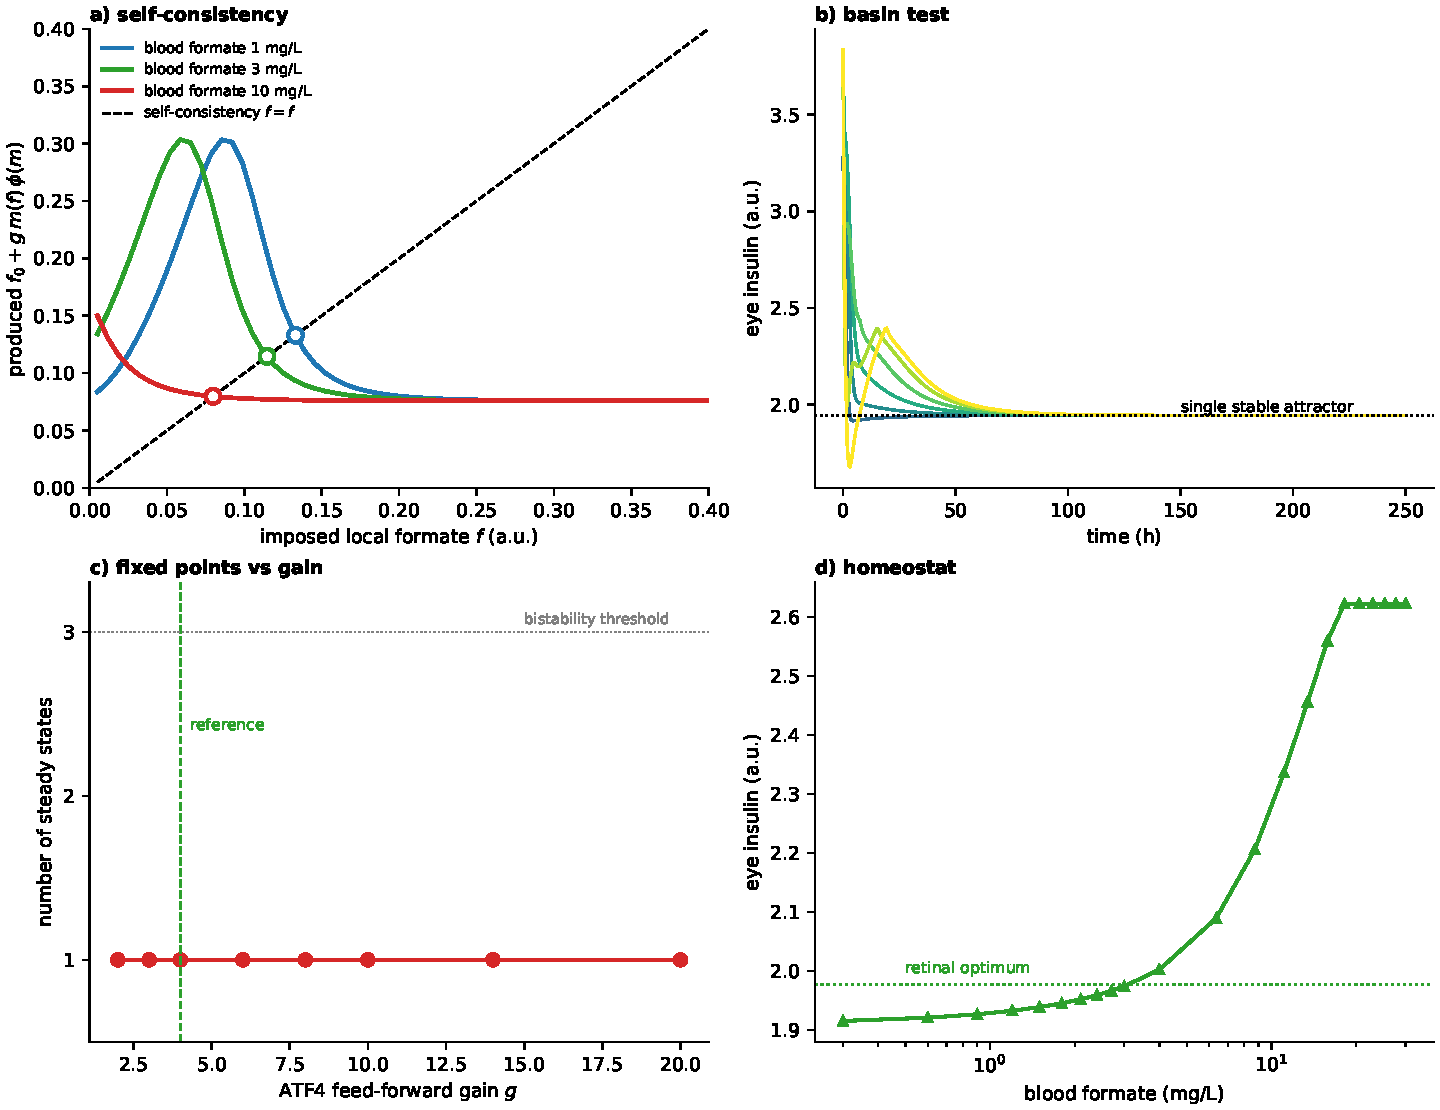
\includegraphics[width=\linewidth]{figS_eye_bifurcation.pdf}
  \caption{\textbf{The regulated eye feed-forward is monostable.}
  (A) Self-consistency~\eqref{eq:selfcons}: produced vs.\ imposed local formate at
  three blood-formate levels; each curve crosses the diagonal exactly once (open
  circles) --- a single fixed point. (B) Basin test: trajectories from initial
  states $0.2\times$ to $10\times$ all converge to one stable attractor.
  (C) Number of steady states vs.\ feed-forward gain: monostable throughout,
  including five-fold the reference gain (dashed) --- no bistability.
  (D) The resulting single-valued homeostat: eye insulin vs.\ blood formate,
  buffered near the retinal optimum across the physiological range and rising to
  excess only above it.}
  \label{fig:bif}
\end{figure}

\textbf{Intravitreal MTHFD2 inhibitor.} MTHFD2 is the mitochondrial entry enzyme
of the pathway that produces the retina's local formate. An intravitreal MTHFD2
inhibitor is modelled as a factor $\eta\in[0,1]$ (fraction of activity remaining;
$\eta=1$ uninhibited, $\eta=0$ full block) scaling the \emph{local} mitochondrial
formate only,
\begin{equation}
f_{\mathrm{mito}}=\eta\,\big[\mathrm{EYE\_FMITO}+g\,m\,\phi(m)\big],
\end{equation}
while blood-delivered formate (the barrier-crossing term $k_F(\mathrm{form}_x-form)$
inside the $\beta$-cell derivatives) is untouched. Sweeping $\eta$ shows the
therapy is conditional: for an insulin-\emph{excess} retina (lean secretion-defect
overflow, hyperglycaemic) partial inhibition (${\sim}70$--$80\%$) walks local
insulin back through the optimum and net health rises from ${\sim}0.30$ to
${\sim}0.42$, whereas for a formate-\emph{deficient} retina the same inhibition
deepens the deficiency (health ${\sim}0.42\to0.19$). Against a methanol formate
flood the inhibitor has no effect (the toxic formate is blood-borne, bypassing
MTHFD2): eye insulin and health are identical with and without the drug at
intoxication levels. This is generated by \texttt{make\_mthfd2.py}.

\textbf{Insulin-production (mTOR) inhibitor.} Insulin synthesis is mTOR-driven, so
an mTORC1 inhibitor (rapamycin/sirolimus, which reduces $\beta$-cell proinsulin
biosynthesis) is modelled by the $\beta$-cell $\mathrm{mtor\_mult}<1$ threaded
through \texttt{eye\_state\_ff}; it caps the mTOR-driven insulin translation
\emph{downstream} of formate and purine sensing (and relaxes the S6K feedback and
local feed-forward, which are also mTOR-scaled). Unlike the MTHFD2 inhibitor, it
therefore acts on a blood-borne overload: under a methanol formate flood a
${\sim}50\%$ mTOR inhibition holds eye insulin at the optimum and net retinal
health at its peak (${\sim}0.42$) across the whole methanol range (versus the
${\sim}0.24$ insulin-excess floor untreated), with a therapeutic window (peak near
$50\%$; over-inhibition overshoots into deficiency) and little effect on the
physiological eye (a proportional cap preferentially clips the saturated excess).
Generated by \texttt{make\_mtor\_inhibitor.py}.

\textbf{Methanol.} The methanol overload analysis uses this insulin-excess route
alone (complex-IV inhibition switched off): raising blood formate to the
symptomatic ($>50$~mg/L) and lethal ($>500$~mg/L) range drives local insulin past
the optimum into pathology. The regulated eye is protected across the physiological
range (health at its peak $\sim0.42$) but, once external formate floods in, both
the regulated and blood-dependent eyes collapse to the same insulin-excess health
floor ($\sim0.24$) --- an acute overload that overwhelms regulation, not a chronic
mis-set of local insulin.

% ===========================================================================
\section{Dietary meta-analysis mapping}\label{sec:diet}

Per-serving formate contents are mapped to model dietary intake and each food's
blood-formate prediction (\texttt{make\_diet.py}). Whole-food contents (creatine
$1000$~mg, red meat $700$~mg, fruit juice $70$--$600$~mg/L) are from
\textit{The Spice of Life} (p.~53); caffeine/aspartame drinks and medications use
the formate-generation potential of Pietzke, Meiser \& Vazquez (2020, Table~2) ---
the formaldehyde released by caffeine/aspartame demethylation, taken to full
conversion to formate (formate per serving $=$ formaldehyde$_{\mathrm{mmol}}\times
46.03$), giving e.g.\ diet cola ${\sim}43$~mg, brewed coffee ${\sim}31$~mg, regular
cola ${\sim}8$~mg, caffeine pill ${\sim}47$~mg. A serving's formate is treated as a
daily intake, $D_{\mathrm{diet}}=3\times10^{-5}\times(\text{mg})$~mM/h (so
$1$~g/day maps to the normal intake $0.030$~mM/h), and run through the lean-healthy
fixed point of \S\ref{sec:adip}. These are compared against pooled relative risks
of incident type~2 diabetes per serving (coffee, sugar-sweetened and diet cola,
100\% fruit juice, red meat, creatine). The correlation between a food's formate
content and its diabetes effect is essentially zero ($r=-0.03$): because the
$\beta$-cell is formate-replete, dietary formate raises blood formate but leaves
plasma insulin and fasting glucose flat, and the model's only appreciable dietary
response is the modest, sub-optimal rise in eye insulin.

% ===========================================================================
\section*{References}
\small
\begin{enumerate}\itemsep1pt
  \item Vazquez A. An allosteric metabolite glue couples AICAR inversely to
  one-carbon availability (submitted) --- the Formate--NUDT5 purine/energy core
  reused here.
  \item Witus \textit{et al} (2026) Metabolite glues as a means of purine sensing
  and chemotherapeutic response. \textit{Nature} (the PPAT--NUDT5 PRPP/AMP glue
  data).
  \item Detimary P \textit{et al} (1998) The changes in adenine nucleotides
  measured in glucose-stimulated rodent islets. \textit{J Biol Chem} 273:33905.
  \item Gooding JR \textit{et al} (2015) Adenylosuccinate is an insulin
  secretagogue derived from glucose-induced purine metabolism. \textit{Cell Rep}
  13:157.
  \item Ni Q \textit{et al} (2017) Raptor regulates functional maturation of
  murine beta cells. \textit{Nat Commun} 8:15755.
  \item Tsushima Y \textit{et al} (2013) Uric acid secretion from adipose tissue
  and its increase in obesity. \textit{J Biol Chem} 288:27138.
  \item Kasahara K \textit{et al} (2023) Gut bacterial metabolism contributes to
  host global purine homeostasis. \textit{Cell Host Microbe} 31:1066--1081.
  \item Vazquez A (2020) The urate cycle and obesity. Preprint
  (ResearchGate 341427356).
  \item Pietzke M, Meiser J, Vazquez A (2020) Formate metabolism in health and
  disease. \textit{Mol Metab} 33:23--37.
\end{enumerate}

\end{document}
